\graphicspath{{./img/}}

Nuestra Hipotesis a la hora de experimentar, es que, utilizar el modelo SIMD con operaciones SSE, nos da una mayor performance a la hora de desarrollar nuestros algoritmos. El hecho de poder procesar varios datos a la misma vez, nos permite ahorrarnos tiempo de ejecucion y cantidad de iteraciones en nuestros algoritmos.
Realizamos distintas corridas de nuestro codigo, tanto en ASM, como en C con las correspondientes optimizaciones que nos permite el compilador. De esta manera pudimos respaldar nuestra hipotesis con resultados concretos.

\subsection{solver\_lin\_solve}

\subsection{solver\_set\_bnd}

En solver$\_$set$\_$bnd se hicieron 4 gráficos para comparar ASM y C con los distintos tamaños, que son iguales a los tamaños de las imágenes de la cátedra. El solver tiene 2 matrices de floats, que son las que utilizamos para hacer los experimentos en este caso. Si bien el $b$ se cambió en cada iteración para que el procesador no cachee los experimentos y tengamos tiempos medianamente razonables, no se graficó ya que no influye en el algoritmo.
Los pasos para los experimentos fueron los siguientes:
Por cada tamaño, en total 6, se hicieron 750 iteraciones. En cada iteración se corre un código diferente(ASM, C), con una matriz diferente (v o u) y con b diferente (0, 1, 2) a la iteración inmediata anterior. En todos los siguientes casos se utiliza la mediana como mediana.
Todo esto se vuelca en un csv, donde por python, con las bibliotecas NumPy y Matplotlib terminamos haciendo los gráficos. 

\begin{figure}[h]
  \centering
  	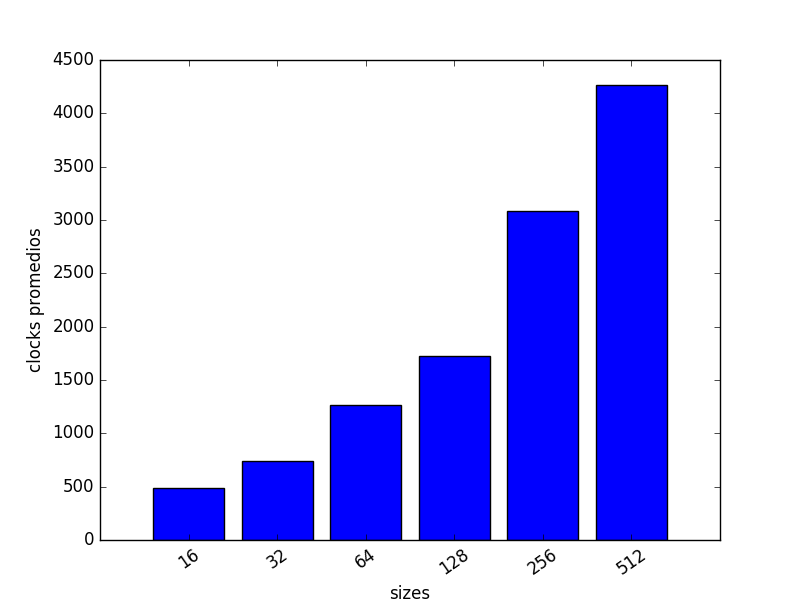
\includegraphics[width=.6\linewidth]{ClocksASMU.png}
  	\caption{Código ASM con matriz U}
  	\label{fig:ASMU}
\end{figure}

\pagebreak

\begin{figure}[h]
  \centering
  	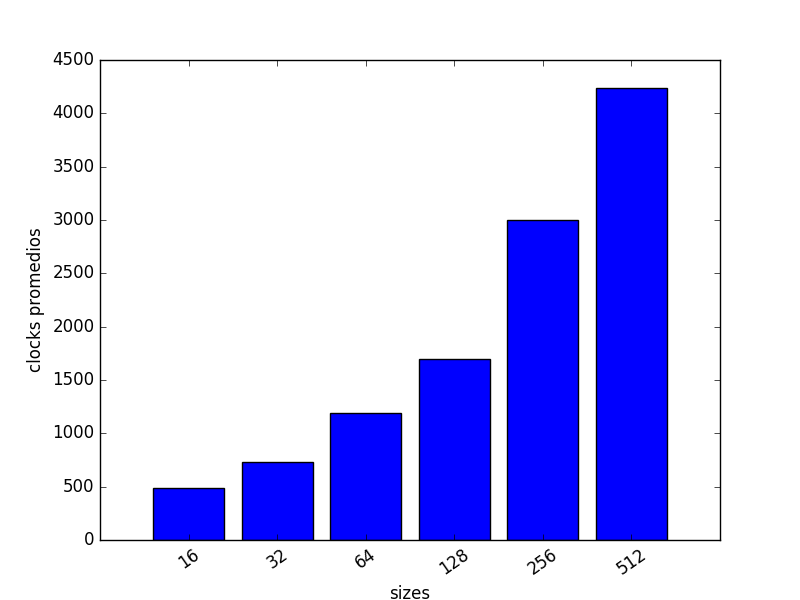
\includegraphics[width=.6\linewidth]{ClocksASMV.png}
  	\caption{Código ASM con matriz V}
  	\label{fig:ASMV}
  \centering
  	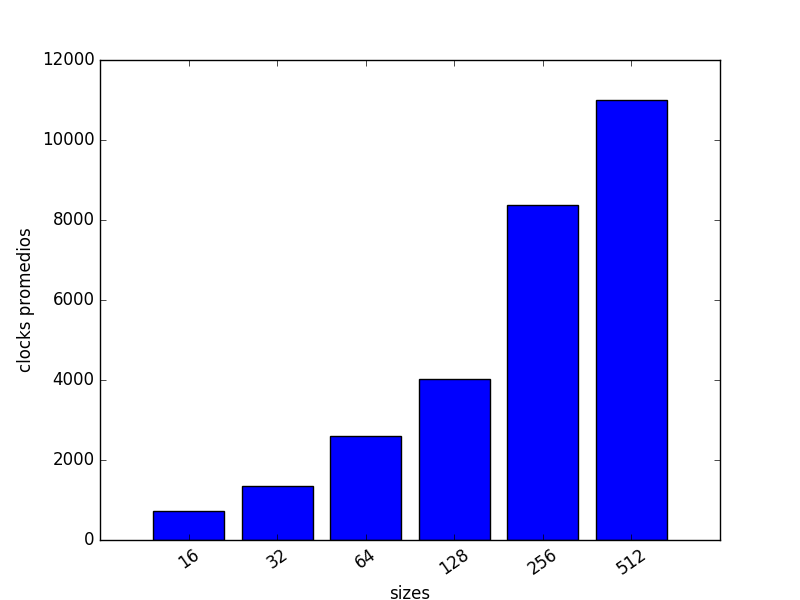
\includegraphics[width=.6\linewidth]{ClocksCU.png}
  	\caption{Código C con matriz U}
  	\label{fig:CU}
\end{figure}

\begin{figure}[h]
  \centering
  	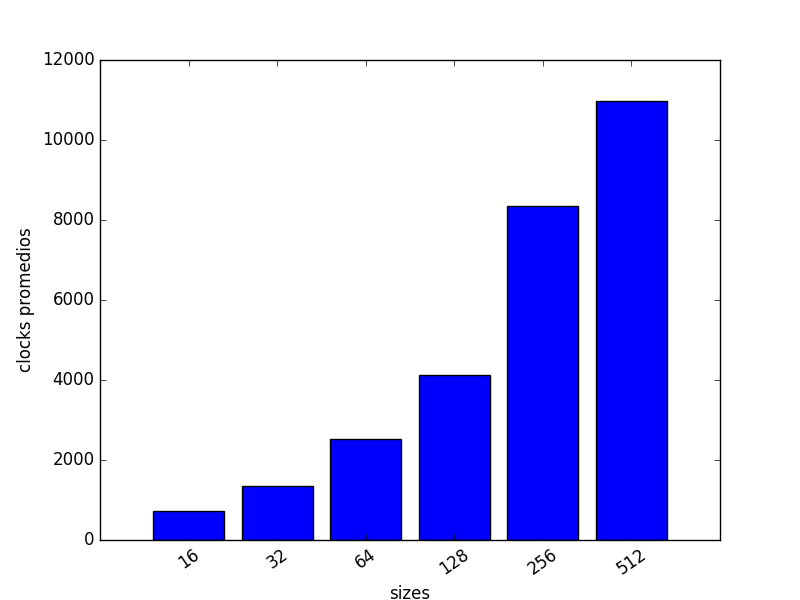
\includegraphics[width=.6\linewidth]{ClocksCV.png}
  	\caption{Código C con matriz V}
  	\label{fig:CV}
\end{figure}

\pagebreak

\subsection{solver\_project}

El solver 